\documentclass[../main.tex]{subfiles}
\begin{document}
\subsection{What is the core idea of deep learning? How does it differ from shallow learning?}

The core idea of deep learning is to have several hidden layers to describe complicated functions. This enables more complex representations, with the disadvantage of more computing power needed, as well as overfitting. \autoref{fig:deep_example} shows a diagram of a deep neural network, where $\mathbf{u}=\{u_1, u_2\}$, $\mathbf{v}=\{v_1, v_2\}$, and the cloud denotes hidden layers. 

A shallow network contains fewer, if any, hidden layers. It can represent all functions, but the number of parameters expands rapidly with the complexity of the function. It is less prone to overfitting. A shallow network is displayed in \autoref{fig:shallow_example}, where $\mathbf{u}=\{u_1, u_2\}$ is the only hidden layer.

\begin{figure}
    \centering
    \begin{subfigure}[b]{0.48\textwidth}
    	\centering
        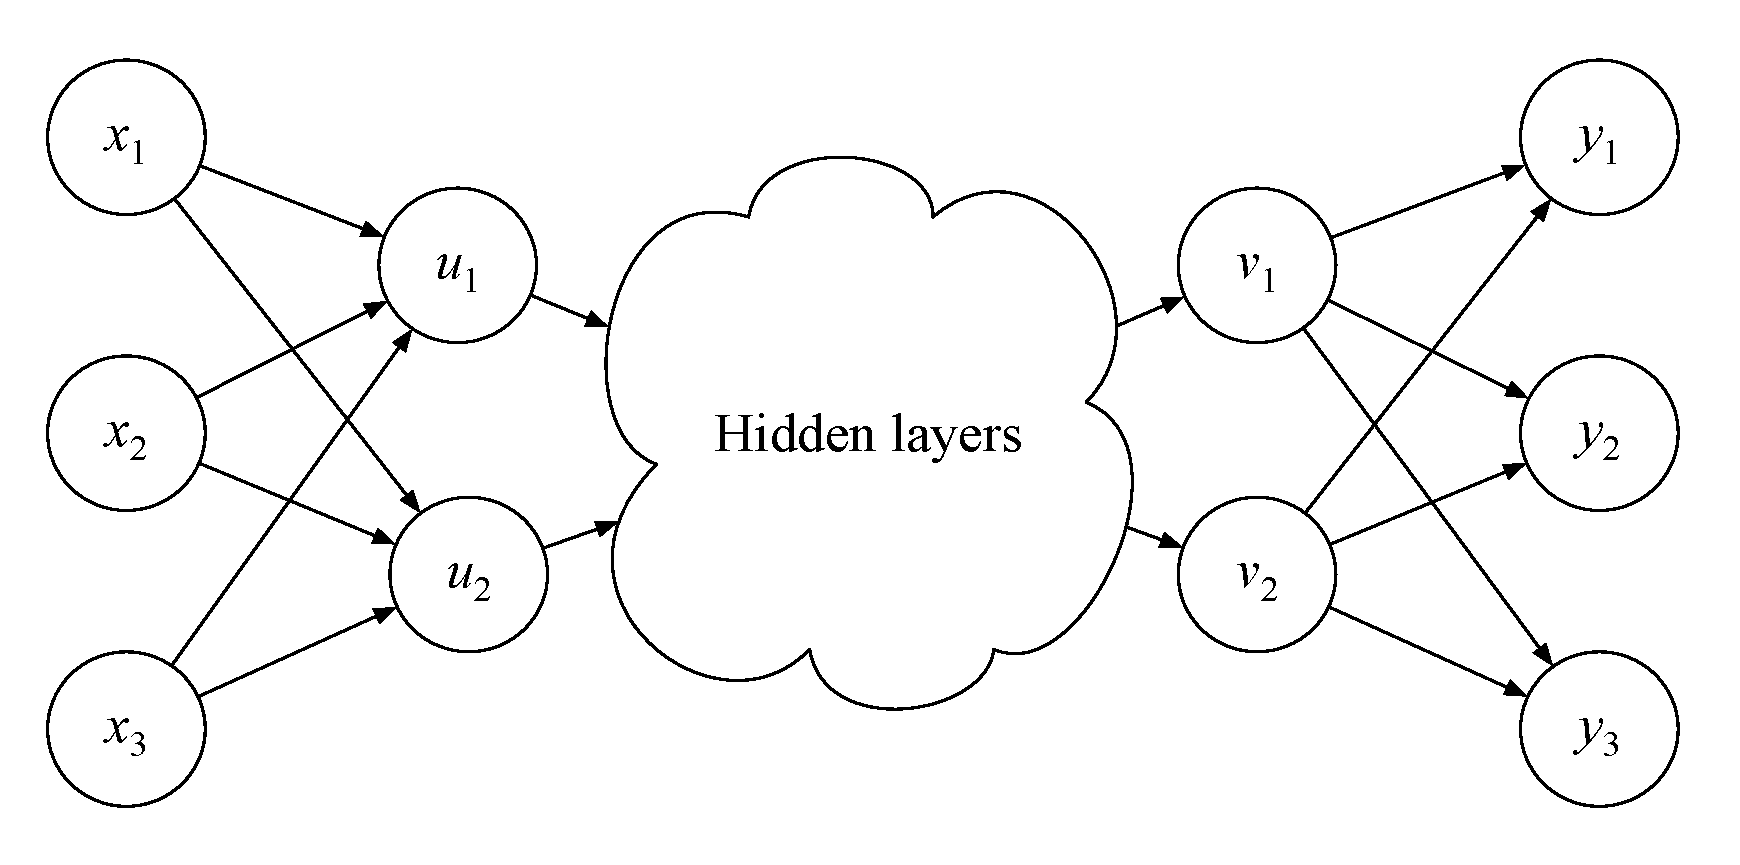
\includegraphics[height=3cm]{figures/theory/deep_network}
        \caption{Example of a deep network}
        \label{fig:deep_example}
    \end{subfigure}
    ~
    \begin{subfigure}[b]{0.48\textwidth}
    	\centering
        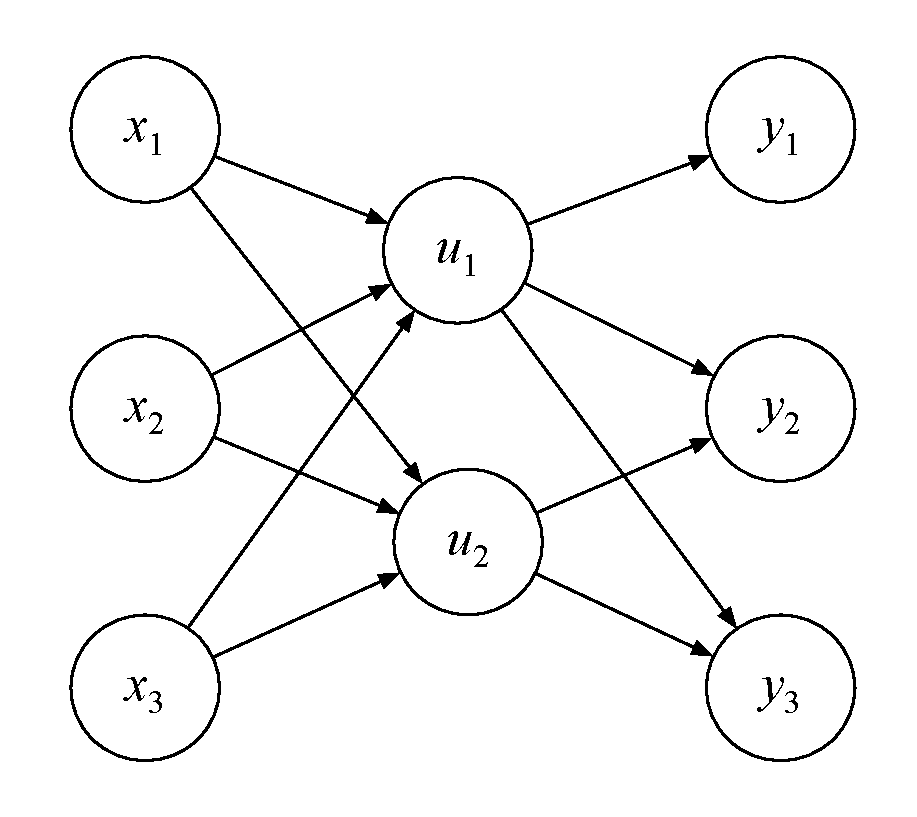
\includegraphics[height=3cm]{figures/theory/shallow_network}
        \caption{Example of a shallow network}
        \label{fig:shallow_example}
    \end{subfigure}
    \caption{Deep and shallow networks.}\label{fig:deep_shallow}
\end{figure}


\subsection{}

\begin{subfigure}
	\centering
    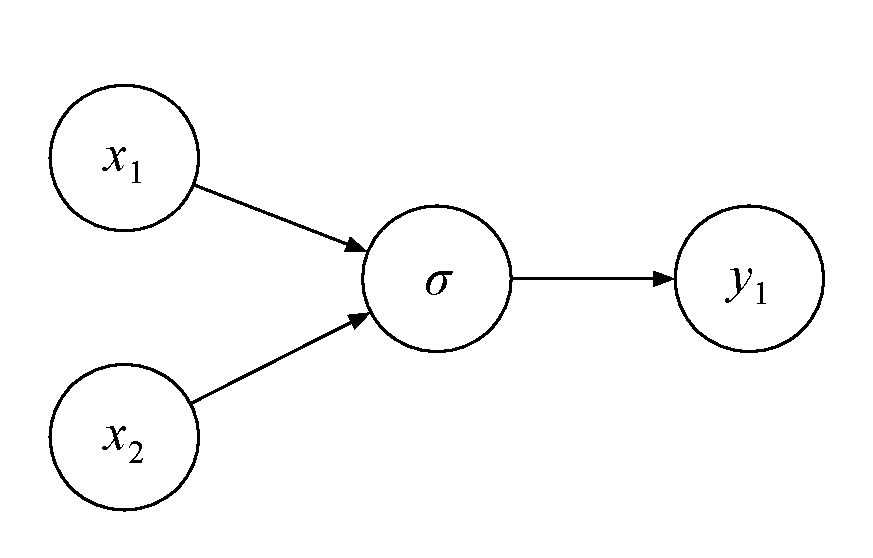
\includegraphics[height=3cm]{figures/theory/log_network}
    \caption{Example of a deep network}
    \label{fig:log_example}
\end{subfigure}


\end{document}